% \lipsum[2-3]

\section{Motivation}
\setauthor{Arsham Edalatkhah}

In der heutigen sich schnell entwickelnden Welt verändert die Urbanisierung die Art und Weise, wie die Menschen leben, rapide, was zu einer zunehmenden Anonymität und Unverbundenheit innerhalb der Nachbarschaft führt. Das Team Nochba hat diese Herausforderung erkannt und eine Möglichkeit gefunden, Gemeinschaften zusammenzubringen und die Verbindung, Zusammenarbeit und Unterstützung zwischen Nachbarn zu fördern.

Durch die Entwicklung einer Social-Media-App, die speziell für die Kommunikation in der Nachbarschaft entwickelt wurde, hofft das Team Nochba, die Kluft zwischen den Gemeindemitgliedern zu überbrücken und ihnen zu helfen, Sprachbarrieren, kulturelle Unterschiede und die Herausforderungen des modernen Stadtlebens zu überwinden. Das Team möchte die Nachbarschaft, wie man sie in den Dörfern kennt, in die Städte bringen.

\section{Aufgabenstellung}
\setauthor{Arsham Edalatkhah}

Das Team Nochba hat sich auf die Entwicklung einer auf die Nachbarschaft fokussierten Social-Media-App konzentriert, die den Zusammenhalt der Gemeinschaft stärken und den Austausch von Ressourcen unter den Nachbarn erleichtern soll. Das Team hat eine Reihe von Meilensteinen festgelegt, um einen systematischen und effizienten Ablauf des Projekts zu ermöglichen.

Das Team hat sich auf die folgenden Meilensteine geeinigt:

\begin{itemize}
    \item {Entwurf eines Prototypen für die Benutzeroberfläche.}
    \item {Festlegung der Systemarchitektur und Überprüfung der technischen Machbarkeit.}
    \item {Implementierung eines Minimum Viable Product (MVP) mit Funktionen wie Login, Feed, Beitragserstellung, Filter und Chat-Funktion.}
    \item {Ein Minimum Loveable Product (MLP) entwickeln, das Registrierung, Suche, Kontoeinstellungen, Aktivitäten-Tab, Übersetzung, Kommentarfunktion, mehrere Beitragskategorien und ein Reportsystem umfasst.}
    \item {Vervollständigung der Implementierung aller geplanten Funktionen.}
    \item {Beseitigung von Schwachstellen durch Kundenfeedback und Bugfixing.}
    \item {Fertigstellung und Einreichung des Diplomarbeitsprojekts.}
\end{itemize}

Das Team Nochba beabsichtigt, die Arbeit an diesem Projekt auch nach Abschluss der Diplomarbeit fortzusetzen und die App zu verfeinern und zu erweitern, um die Communities besser zu unterstützen und die Verbindung zwischen den Nachbarn zu fördern.

\section{Projektresultate und wichtige Meilensteine}
\setauthor{Arsham Edalatkhah}

\begin{itemize}
    \item \textbf{Auszeichnungen:}
          \begin{itemize}
              \item \textbf{\#1 Platz Linz hACkT Event X Innovationshauptplatz}
              \item \textbf{\#1 Platz mPreneur Austria Contest X ICT4D.at}
              \item \textbf{\#1 Platz Immotopia Innovation Award}
              \item \textbf{\#3 Platz Spusu Innovation Award (Wien)}
              \item \textbf{Siegerteam bei mPreneur School Ohrid X World Summit Award}
              \item \textbf{Projektpräsentation für den Bürgermeister von Linz und die Magistratsdirektorin}
          \end{itemize}
    \item \textbf{Teilnahme an Workshops:}
          \begin{itemize}
              \item \textbf{Workshop Planet Linz Days}
              \item \textbf{Workshop Jugendhackt Österreich}
              \item \textbf{Workshop Project-Forge ICT4D.at}
          \end{itemize}
    \item \textbf{Medienauftritte:}
          \begin{itemize}
              \item \textbf{UNESCO Internet4trust Konferenz}
          \end{itemize}
    \item \textbf{Bevorstehende Events:}
          \begin{itemize}
              \item \textbf{World Summit Award (Graz)}
          \end{itemize}
    \item \textbf{Wichtige Meilensteine:}
          \begin{itemize}
              \item \textbf{Veröffentlichung von der \textit{Nochba App} im Play Store}
          \end{itemize}
\end{itemize}

Seit Beginn des Diplomarbeitsprojekts hat sich das Nochba Team auf die Entwicklung einer App mit dem Fokus auf soziale Aspekte im Bereich \textit{Ressourcen-Sharing} und \textit{Community Building} konzentriert. Das Ziel des Teams war es, ein Konzept zu entwerfen, das es ermöglicht, auch nach Abschluss der Diplomarbeit einen wertvollen Beitrag für die Gesellschaft zu leisten. Um die IT-Kenntnisse zu vertiefen und von Mentoren und Branchenexperten mehr über das Thema der sozialen Innovation zu erfahren, entschied sich das Team, an einer Reihe von Wettbewerben und Veranstaltungen teilzunehmen.

Durch diese Erfahrungen konnte das Team Nochba eine solide Grundlage für das Projekt schaffen und war davon überzeugt, dass dies ein fundamentaler Bestandteil der Vision sein wird, die das Team zu erfolgreichen Ergebnissen führen wird. Die Kompetenz des Teams im Bereich der nachhaltigen Innovation und sozialen Unternehmerschaft wurde durch die Teilnahme an diesen Wettbewerben unterstrichen.

\begin{itemize}
    \item \textbf{Linz-hACkT:}
          \begin{itemize}
              \item \textbf{11. bis 13. März 2022}
          \end{itemize}
\end{itemize}

Während des dreitägigen Linz Hackathon-Events \cite{LinzInnovationshauptplatz} hatte das Team Nochba fünf Mentoren aus verschiedenen Bereichen der IT-Industrie in Österreich und Deutschland, mit denen Coaching-Sessions geplant wurden. Diese Mentoring-Sessions halfen dem Team, die Idee nicht nur aus technischer Sicht zu betrachten, sondern auch aus wirtschaftlicher und sozioökonomischer Perspektive zu analysieren. Themen wie Barrierefreiheit und Sicherheit wurden mit erfahrenen Fachleuten aus der Industrie diskutiert, was dem Team einen ersten Überblick über die Vor- und Nachteile des Projekts gab.

Beispielsweise hat das Team gelernt, dass beim Ressourcen-Sharing-Aspekt der App die ausgetauschten Waren beschädigt zurückgebracht oder sogar gestohlen werden können. Die Wahrscheinlichkeit dafür ist jedoch gering, weil die Nachbarn sich untereinander kennen und daher die bereits bestehende soziale Dynamik eine wichtige Rolle spielt. Der Ruf einer Person hängt auch davon ab, in welchem Zustand die ausgeliehene Ware zurückgebracht wird. Die App trägt nicht nur zur Verringerung der Konflikte in der Nachbarschaft bei, sondern fördert auch die Entstehung neuer Freundschaften durch die Ermutigung, anderen Gutes zu tun.

Das Team Nochba hat an dem Wettbewerb Linz hACkT teilgenommen und den ersten Platz erreicht. Dadurch hat das Team die Chance bekommen, gute Beziehungen zur Stadt Linz, zum Innovationshauptplatz Linz und zu Open Common Linz aufzubauen. Am Tag der Preisverleihung erhielt das Team den Linz hACkT-Pokal persönlich von Bürgermeister Klaus Luger.

Seit der Preisverleihung hält das Nochba Team das Innovationshauptplatz-Team ständig über die Fortschritte bei der technischen Weiterentwicklung der App auf dem Laufenden. Einige Monate später hatte das Team die Chance, am 30. Januar 2023 eine Präsentation für Bürgermeister Klaus Luger und die Magistratsdirektorin Ulrike Huemer zu halten. Das Treffen wurde vom Team des Innovationshauptplatzes organisiert und das Ziel war es, einen Zwischenstandsbericht in Form einer Präsentation über die Leistungen während der Diplomarbeit an der HTL Leonding zu liefern.

Die Abbildung \ref{fig:linz-hackt} zeigt die Preisverleihung des Teams Nochba bei Linz hACkT 2022, bei der der Linzer Bürgermeister Klaus Luger anwesend war.

Folgende Abbildung zeigt das Team Nochba bei der Projektpräsentation des Nochba-Apps für den Bürgermeister von Linz und die Magistratsdirektorin am 30. Januar 2023. [Referenz: Abbildung \ref{fig:Project-presentation-linz-mayor}]

\begin{figure}[H]
    \centering
    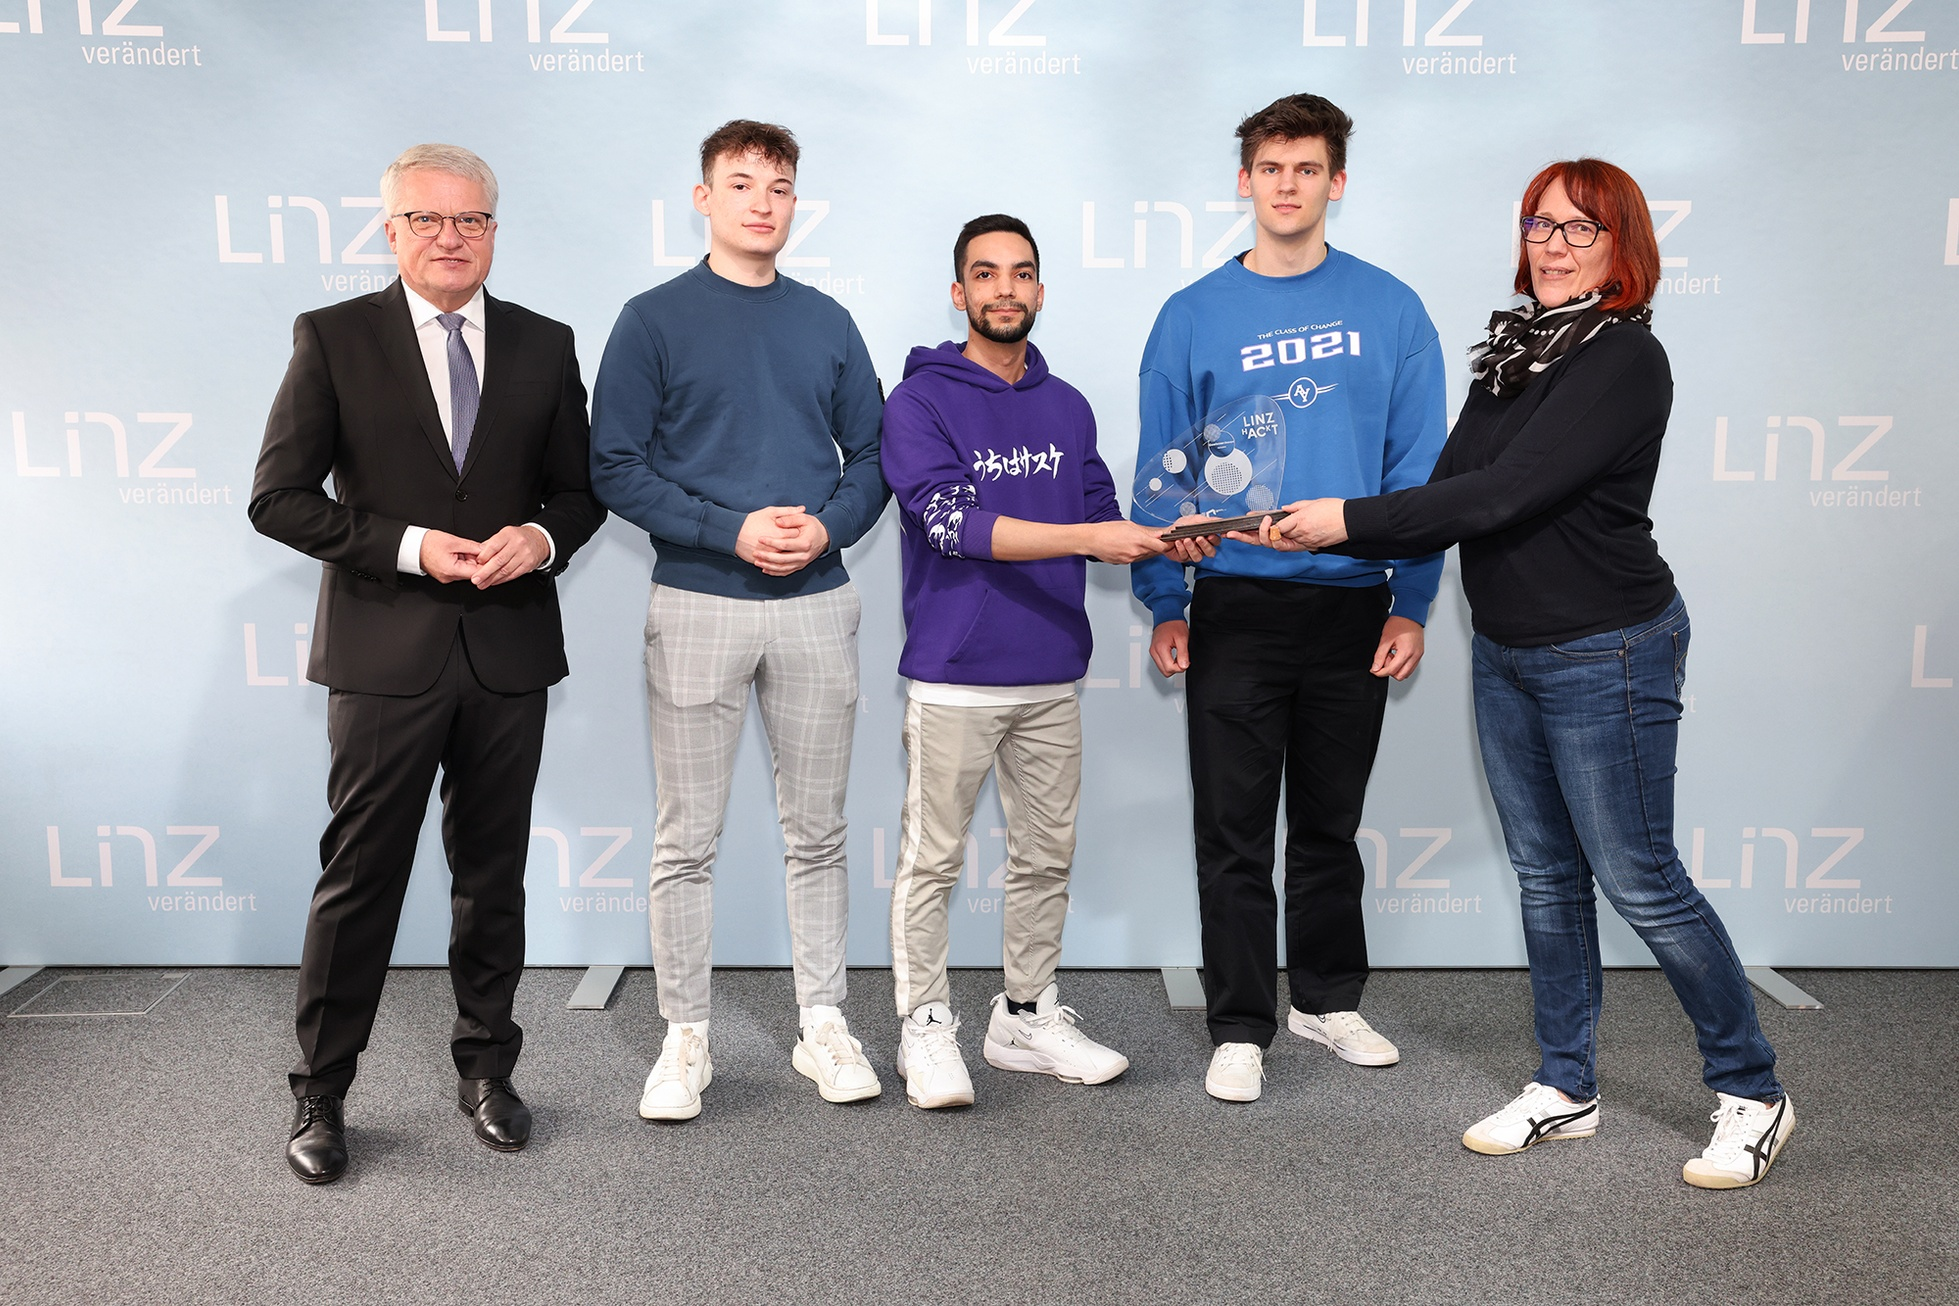
\includegraphics[width=1\textwidth]{pics/Linz-hACkT-2022.jpg}
    \caption{Linz hACkT 2022}
    \label{fig:linz-hackt}
\end{figure}

\begin{figure}[H]
    \centering
    \includegraphics[width=1\textwidth]{pics/B-Präsentation.png}
    \caption{Projektpräsentation für den Bürgermeister von Linz und die Magistratsdirektorin am 30. Januar 2023}
    \label{fig:Project-presentation-linz-mayor}
\end{figure}


\begin{itemize}
    \item \textbf{ICT4D.at X mPreneur Contest Austria:}
          \begin{itemize}
              \item \textbf{22. September 2022}
          \end{itemize}
\end{itemize}

ICT4D.at \cite{ict4d} ist eine Organisation, die im Jahr 2009 gegründet wurde und sich mit der Förderung und Implementierung von Informations- und Kommunikationstechnologien zur Unterstützung von Menschen in Entwicklungsländern beschäftigt. Die Organisation hat den Fokus auf Innovationen mit den Schwerpunkten Bildung, Gesundheit und Sensibilisierung.

Das Nochba-Team entschied sich auf Empfehlung ihres Betreuungslehrers, am mPreneur Contest Austria teilzunehmen, um ein Netzwerk auf österreichweites Niveau aufzubauen und die Vision des Projekts Nochba gemeinsam mit den mPreneur-Mentoren zu verfestigen. mPreneur - Social Mobile Entrepreneurship worldwide - ist ein durch Erasmus+ gefördertes Programm.

Schließlich hat das Nochba Team es geschafft, eines der beiden Siegerteams in diesem österreichweiten Wettbewerb zu werden. Als Siegerteam präsentierte das Team das Projekt vor einer internationalen Jury aus Rumänien, Philippinen, Tansania, Uganda, Singapur, Kenia und Österreich. Alle Teammitglieder erhielten für ihre Leistung ein Teilnahmezertifikat von ICT4D und das Nochba Team hat sich dadurch für die Teilnahme an einem interkontinentalen Wettbewerb in Nordmazedonien qualifiziert.

Diese Abbildung \ref{fig:mpreneur} zeigt das ICT4D.at X mPreneur Contest Austria Event im Jahr 2022, bei dem das Team Nochba als Gewinner ausgezeichnet wurde.

\begin{figure}[H]
    \centering
    \includegraphics[width=1\textwidth]{pics/mPreneur-Austria.JPG}
    \caption{ICT4D.at X mPreneur Contest Austria 2022}
    \label{fig:mpreneur}
\end{figure}

\begin{itemize}
    \item \textbf{Planet Linz Days:}
          \begin{itemize}
              \item \textbf{20. bis 23. Oktober 2022}
          \end{itemize}
\end{itemize}

Der Planet Linz Day \cite{linztourismus} ist eine 3-tägige Veranstaltung mit mehreren Workshops, die von den Gewinnern des Linz Hackathon 2022 gehostet werden. Ziel ist es, der Öffentlichkeit die Konzepte nahezubringen, die die Stadtgesellschaft in Linz beeinflussen werden.

Aufgrund des Erfolges bei der Linz hACkT-Veranstaltung wurde das Nochba-Team eingeladen, am Workshop des Planet Linz Days teilzunehmen. Das Team nutzte diese einmalige Gelegenheit, um eine Umfrage in der Stadt Linz durchzuführen, um herauszufinden, wie sich die BewohnerInnen der Stadt eine Social Media Nachbarschaftshilfe-App vorstellen. Nach der Befragung von insgesamt 50 Personen, um die Perspektive der NutzerInnen zu verstehen,
stellte das Team fest, dass die folgenden sozialen Dynamiken am wesentlichsten sind:


\begin{itemize}
    \item \textbf{Mitteilung}
          \begin{itemize}
              \item \textbf{Frage}
              \item \textbf{Appell}
              \item \textbf{Warnung}
              \item \textbf{Empfehlung}
              \item \textbf{Gefunden}
          \end{itemize}
    \item \textbf{Suche}
          \begin{itemize}
              \item \textbf{Hilfe}
              \item \textbf{Verloren}
          \end{itemize}
    \item \textbf{Ausleihen}
    \item \textbf{Event}
\end{itemize}


Diese Ergebnisse bildeten die Grundlage für die Liste der Kategorien, in denen Beiträge erstellt werden können. Das Team Nochba nutzte diese Ergebnisse und implementierte sie direkt in die Funktion zur Erstellung von Beiträgen in der App, um die App speziell auf die Bedürfnisse der aktuellen Bewohner der Stadt abzustimmen und eine benutzerfreundliche Erfahrung zu schaffen.

\begin{itemize}
    \item \textbf{Jugend hackt Österreich 2022:}
          \begin{itemize}
              \item \textbf{28. bis 30. Oktober 2022}
          \end{itemize}
\end{itemize}

Jugend-Hackt (Quelle: \cite{jugendhackt} ) ist eine Veranstaltung, die von der Non-Profit Organisation \textit{Open Knowledge Austria} organisiert wird. Sie veranstaltet eine Reihe von Hackathons, Events und Workshops. Ziel ist es, Innovation und kreative Teamarbeit unter Jugendlichen im Alter von 12 bis 18 Jahren zu fördern.

Das Team Nochba hat sich für die Teilnahme am Wettbewerb Jugend hackt Österreich 2022 entschieden, weil das Modell der Nochba-App perfekt in das Schema der Veranstaltung passt. Jedes Projekt bekommt die Möglichkeit, seine Projektideen vor den Organisatoren der Veranstaltung zu pitchen. Der Wettbewerb wird aufgezeichnet und kann auf der offiziellen \textit{Dorf TV}-Website und dem offiziellen YouTube-Kanal von Youth Hacks angesehen werden. (Quelle: \cite{youtube-jugendhackt-pitch} )


\begin{figure}[H]
    \centering
    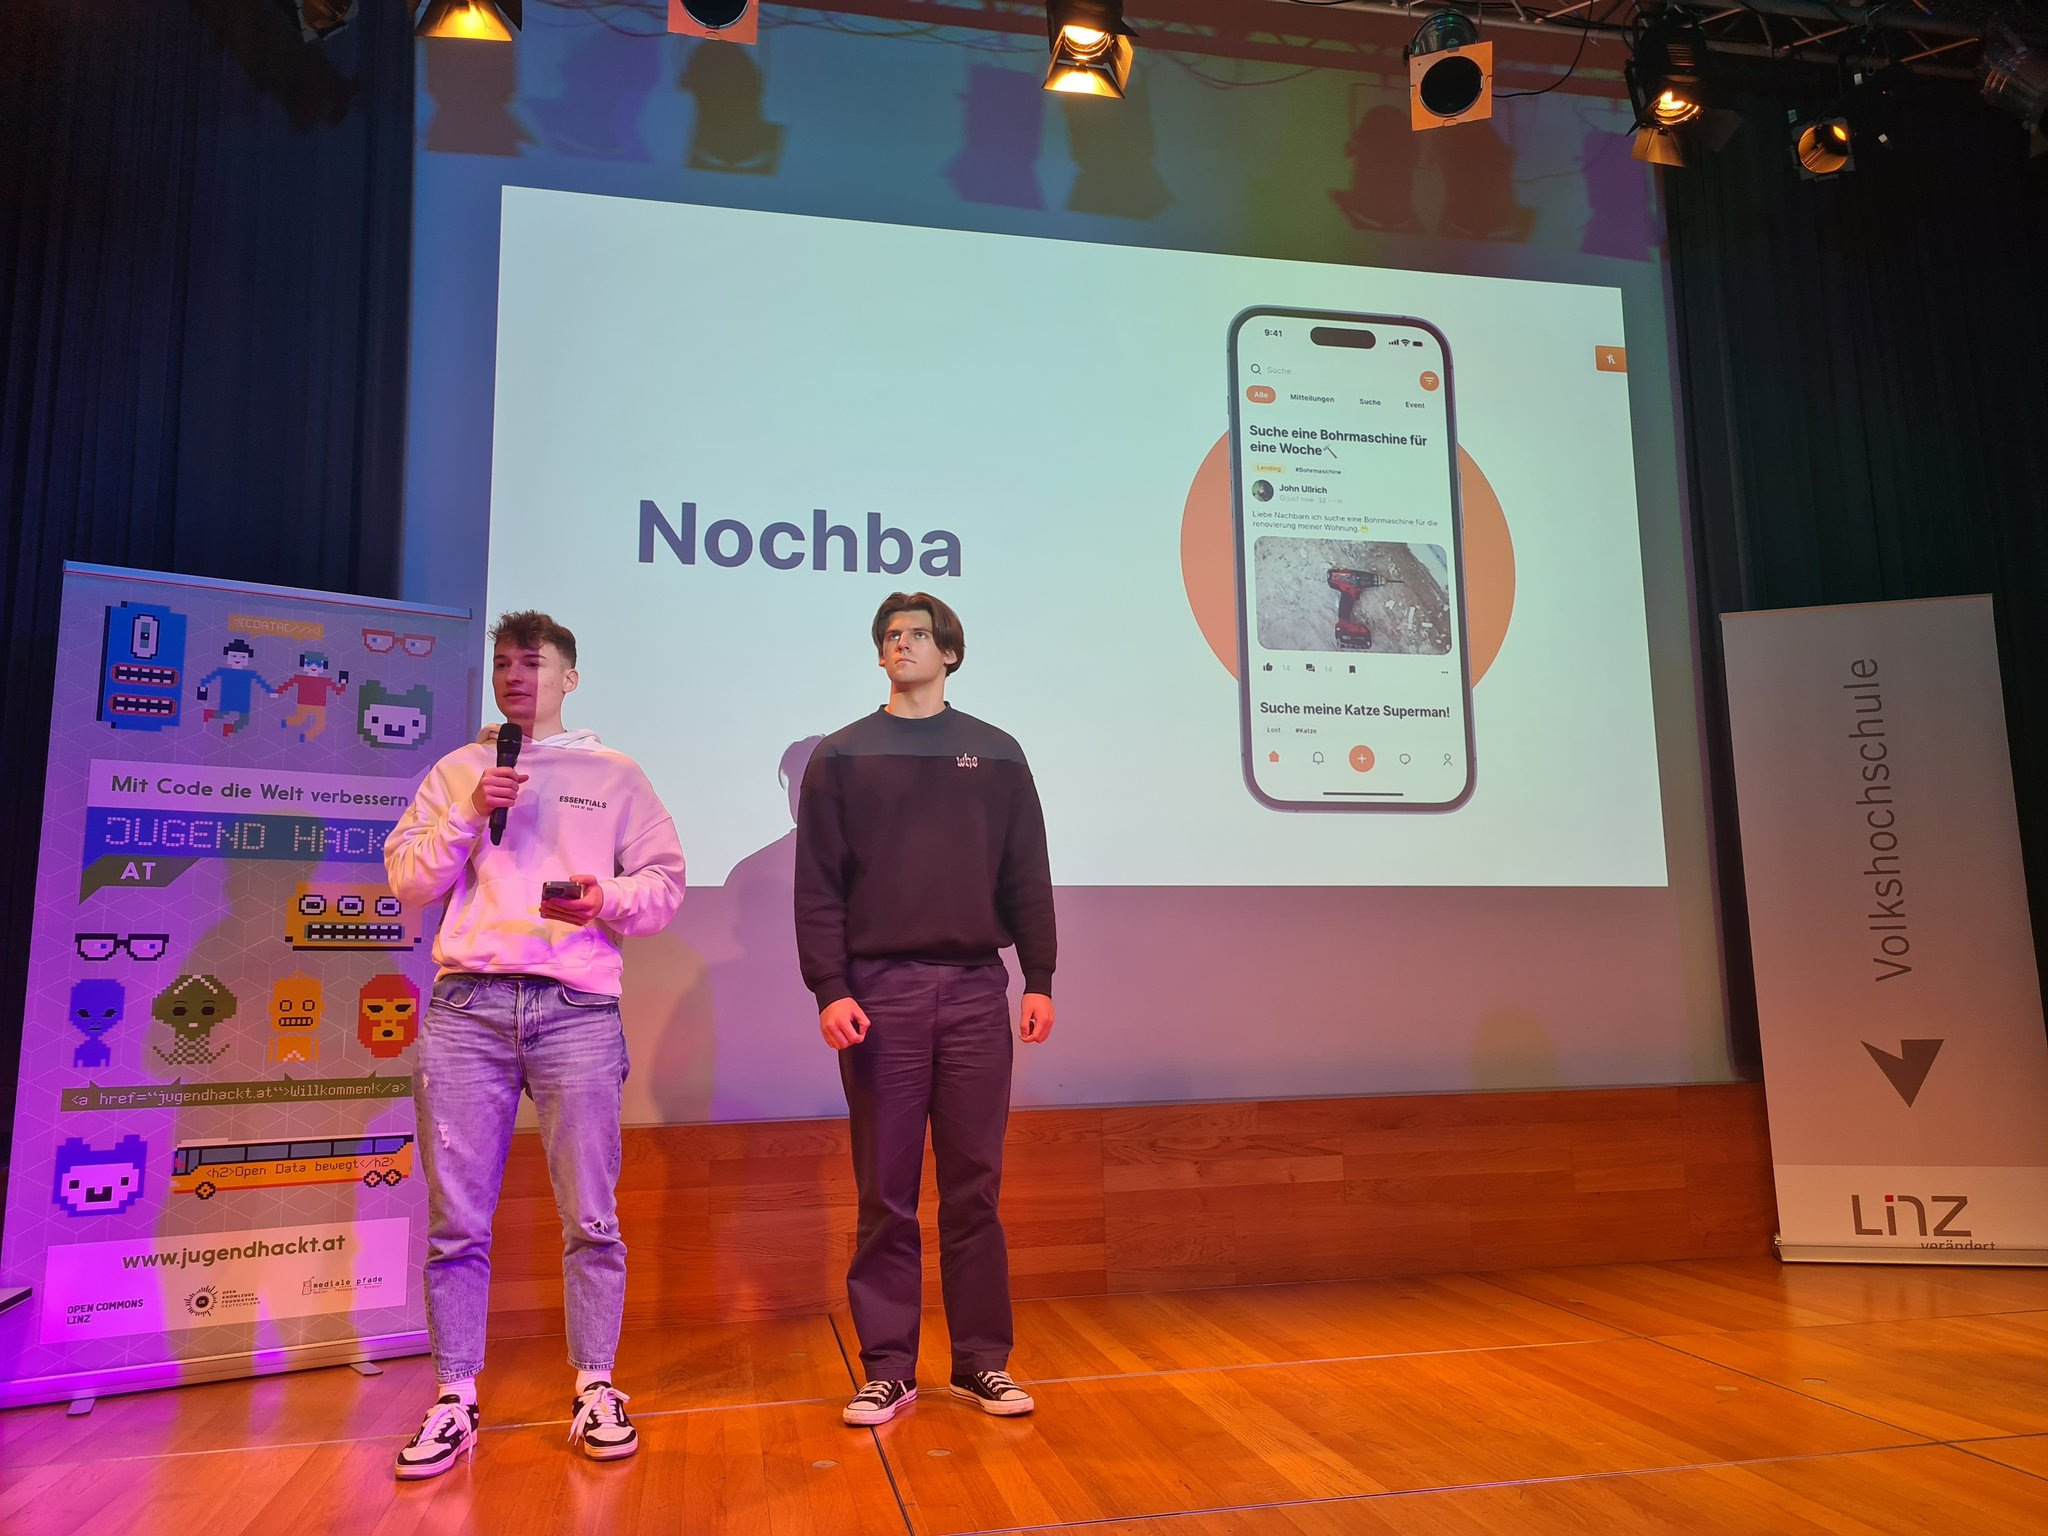
\includegraphics[width=1\textwidth]{pics/JugendHackt.jpeg}
    \caption{Jugend hackt Österreich 2022}
    \label{fig:jugendHackt}
\end{figure}

\begin{itemize}
    \item \textbf{mPreneur School (Ohrid, Nord Mazedonien) X WSA:}
          \begin{itemize}
              \item \textbf{04. bis 09. November 2022}
          \end{itemize}
\end{itemize}

Während der Woche, in der Arsham Edalatkhah an der mPreneur School in Ohrid (Quelle: \cite{mpreneur_training}) teilnahm, wurde er mit dem fortgeschrittenen mPreneur School Programm in Form einer non-formalen Ausbildung betreut. Non-formale Ausbildung umfasst Lernaktivitäten außerhalb des formalen Bildungssystems. Zusammen mit den 16 anderen Teilnehmern aus Asien, Afrika und Europa wurde er von Experten aus verschiedenen Bereichen der Industrie unterrichtet. Die Inhalte der 4 Workshops und der 7 interaktiven Sessions waren Nachhaltiges Entrepreneurship, E-Ethik und soziales Bewusstsein, Künstliche Intelligenz, Big Data und Open Data sowie Virtual Reality und Augmented Reality.

Arsham Edalatkhah ist in dieser Abbildung zu sehen, während er für die 19 World Summit Award Jury Members präsentiert. [Referenz: Abbildung \ref{fig:mPreneurSchool}]

\begin{figure}[H]
    \centering
    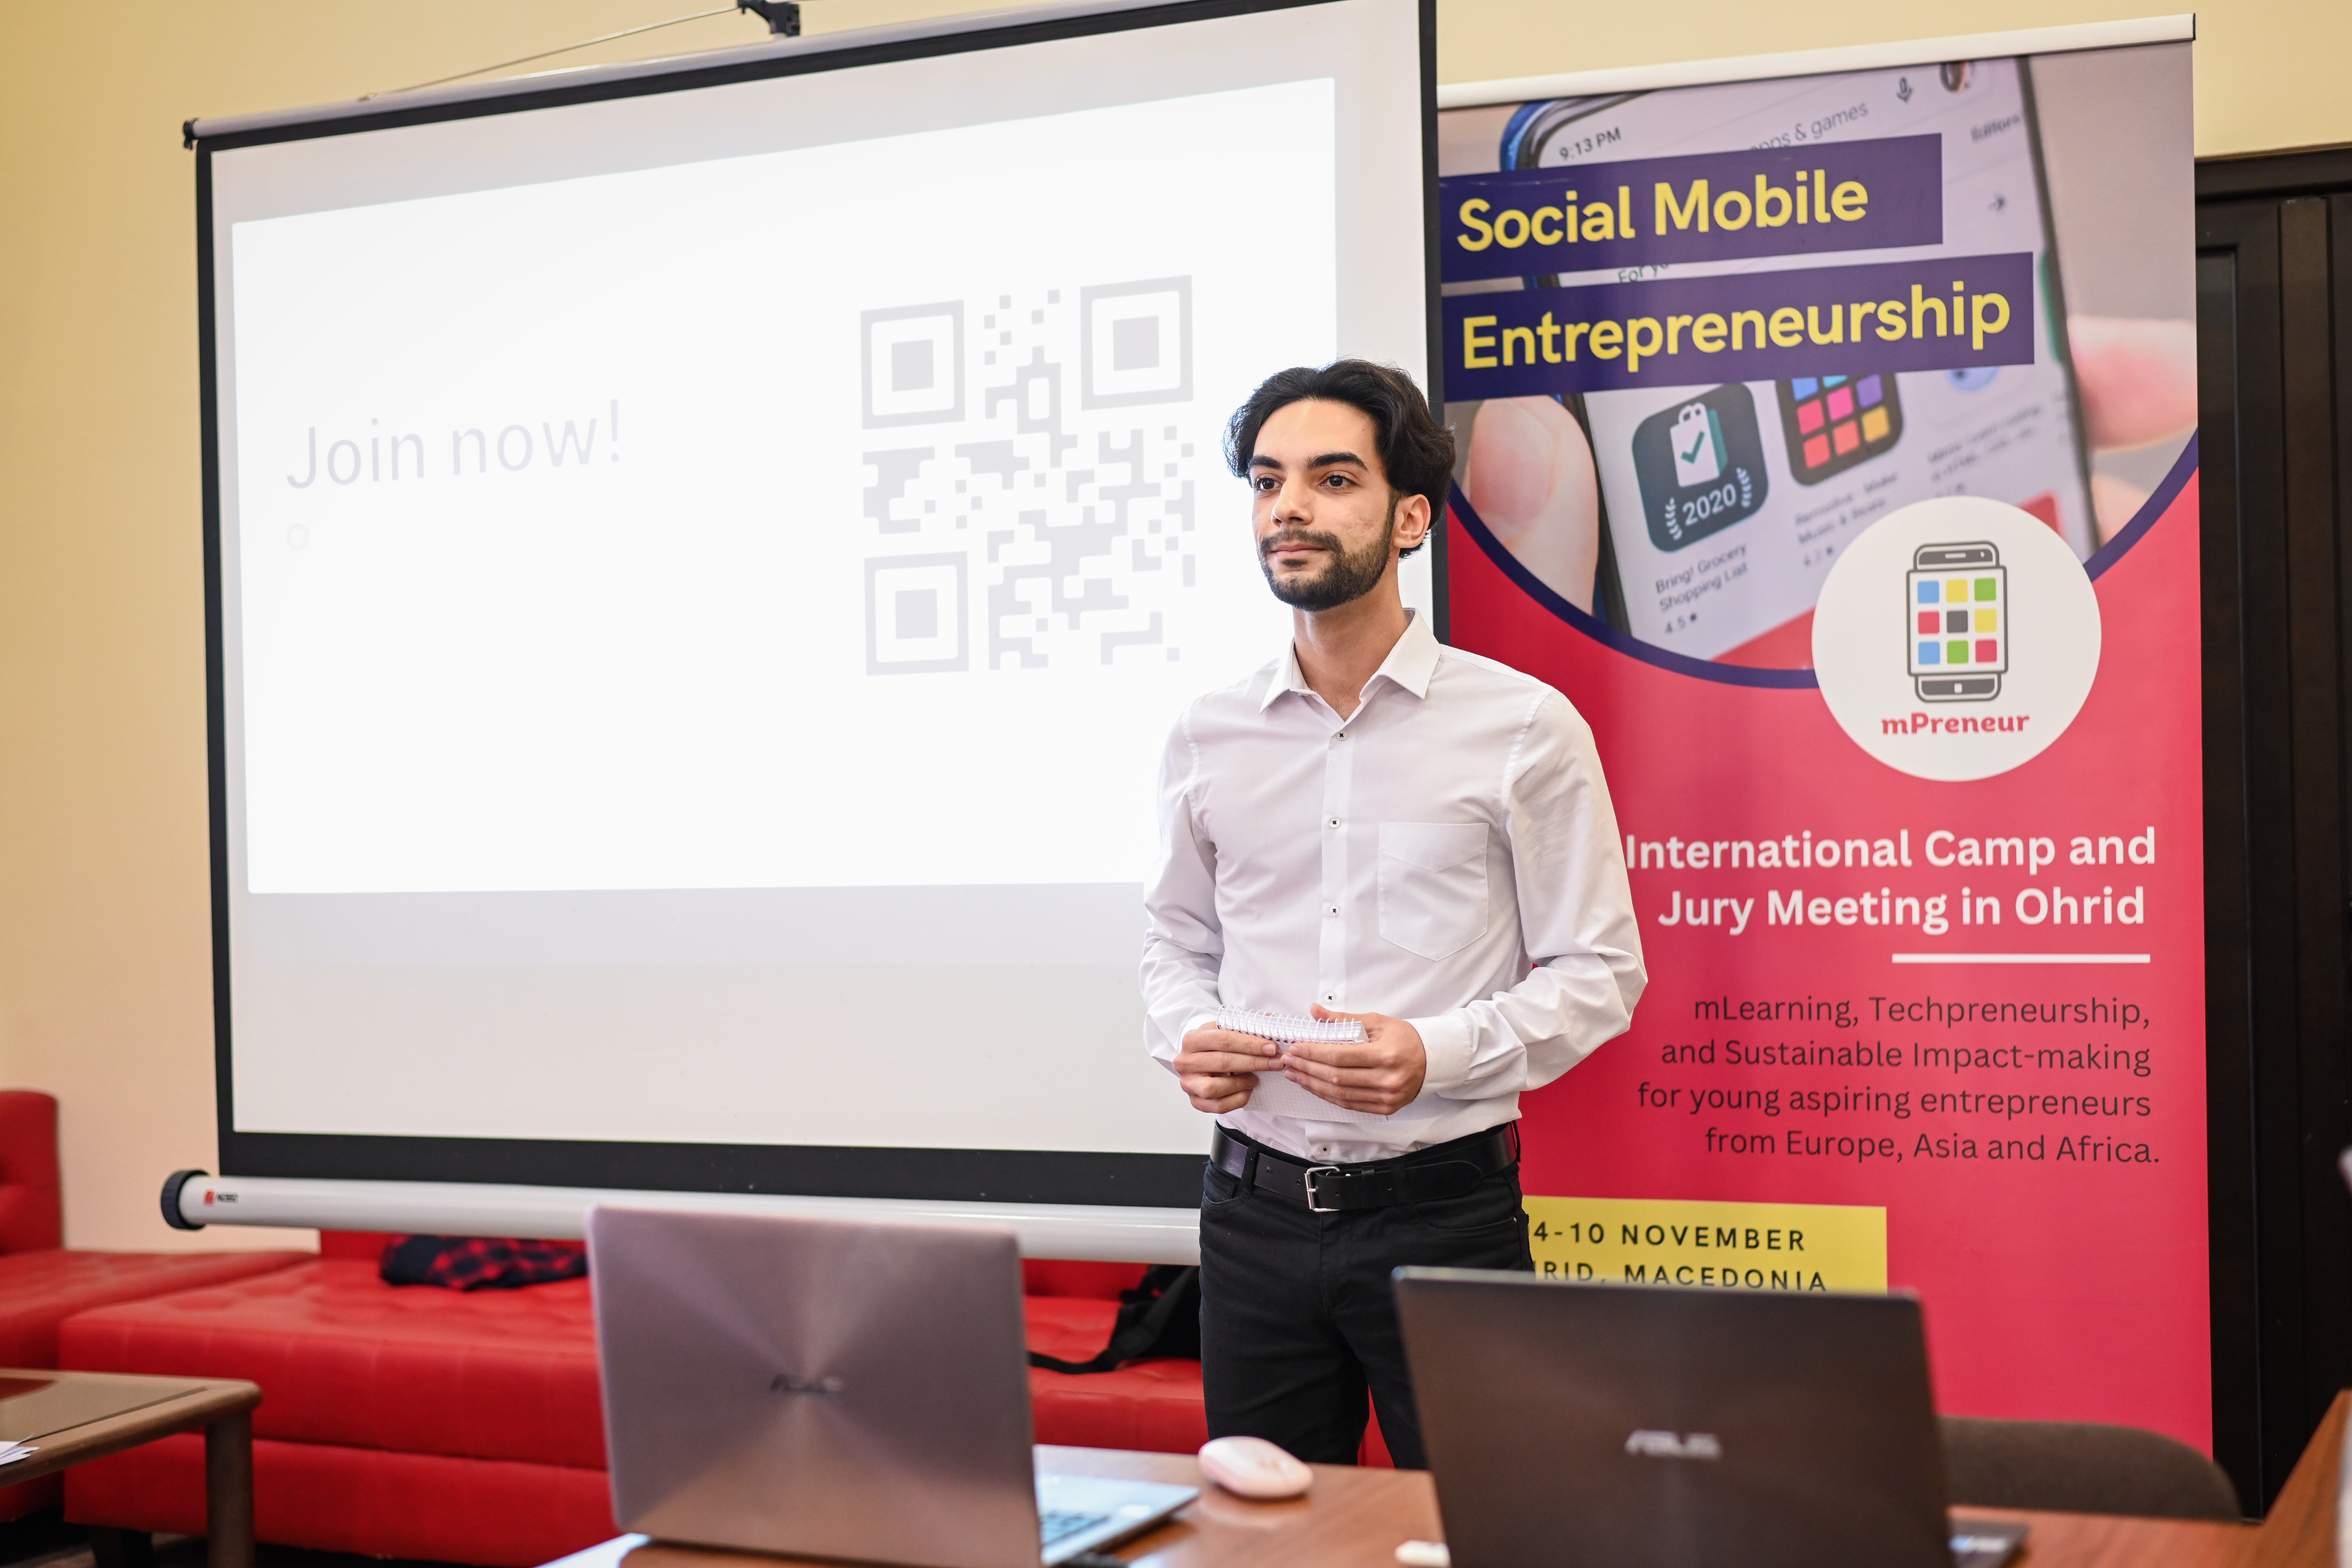
\includegraphics[width=1\textwidth]{pics/mPreneur-2022.JPG}
    \caption{mPreneur School (Ohrid, Nord Mazedonien) X WSA 2022}
    \label{fig:mPreneurSchool}
\end{figure}

WSA (World Summit Award) ist eine Initiative, die im Jahr 2003 von der österreichischen Regierung gegründet wurde. Ziel ist es, mit die Förderung von nachhaltigen digitalen Produkten einen Beitrag zur Erfüllung der 17 UN SDGs (Sustainable Development Goals - United Nations) zu leisten. Die 17 Ziele für nachhaltige Entwicklung \cite{un-sdgs} sollen bis zum Jahr 2030 erreicht werden.

Das Bild in Abbildung \ref{fig:SDG17goals} zeigt die 17 Ziele für nachhaltige Entwicklung der Vereinten Nationen.

\begin{figure}[H]
    \centering
    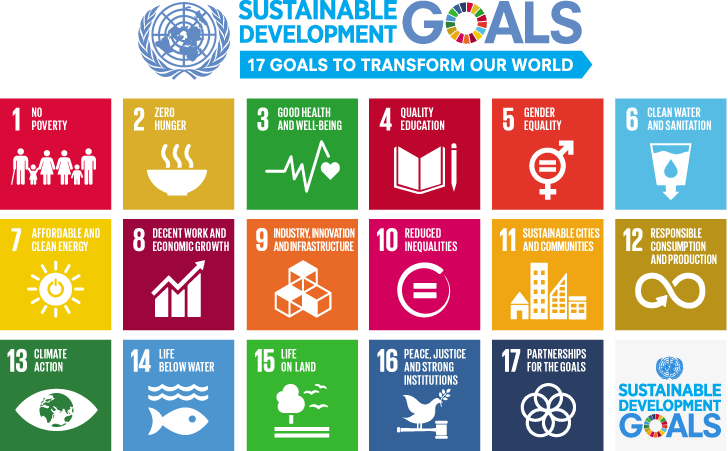
\includegraphics[width=1\textwidth]{pics/SDG-17goals.png}
    \caption{17 Sustainable Development Goals - United Nations (Quelle: \cite{un-sdgs})}
    \label{fig:SDG17goals}
\end{figure}

Alle Länder der Vereinten Nationen haben sich auf diese Agenda für die Zukunft geeinigt. Projekt Nochba ist laut der offiziellen mPreneur Webseite (Quelle \cite{mPreneur-Website}) in 5 der 17 Sustainable Development Goals kategorisiert.

Hier sind die 5 Kategorien:

\begin{itemize}
    \item \textbf{Nachhaltiges Entwicklungsziel Nummer 3:}
          \begin{itemize}
              \item \textbf{Gute Gesundheit und Wohlbefinden}
          \end{itemize}
\end{itemize}

SDG Nummer 3 ist das wichtigste Ziel, und Projekt Nochba ist nun offiziell eines der Projekte, die helfen, Ziel Nummer drei zu erreichen, nämlich Gesundheit und Wohlbefinden für alle Menschen, unabhängig von ihrem Alter.

Studien der Forscher der Brigham Young University zum Thema \textit{Loneliness and Social Isolation as Risk Factors for Mortality: A Meta-Analytic Review} (Quelle \cite{Loneliness-and-Social-Isolation}) zeigen, dass das Gefühl der Einsamkeit dem Rauchen von 15 Zigarren pro Tag entspricht.Die Nochba App trägt zu diesem Ziel bei, indem sie eine sichere virtuelle soziale Dynamik innerhalb einer lokalen Gemeinschaft schafft, in der Menschen unabhängig von ihrem kulturellen Hintergrund und der Sprachbarriere Verbindungen aufbauen oder sogar neue Freundschaften schließen können. So wird Projekt Nochba mit der Social-Media-App für die Nachbarschaft genau dieses Problem der Gesundheit und Einsamkeit aufgreifen.

\begin{itemize}
    \item \textbf{Nachhaltiges Entwicklungsziel Nr. 4:}
          \begin{itemize}
              \item \textbf{Qualitativ hochwertige Bildung}
          \end{itemize}
\end{itemize}

Ziel des SDG Nummer 4 ist es, bis 2030 die Bildungsmöglichkeiten für alle Menschen, unabhängig von ihrem Alter, zu sichern. Vor allem in den Entwicklungsländern, wo es schwierig sein kann, eine qualitativ hochwertige Bildung zu gewährleisten. Ein Aspekt der Qualität der Bildung ist der Zugang zu Nachhilfelehrern.

Die Nochba App trägt zu dieser Herausforderung bei, da sie über eine innovative Funktion verfügt, mit der jeder Nutzer seinen eigenen individuellen Radius festlegen kann, innerhalb dessen er sich mit seinen Nachbarn verbinden kann. Diese Funktion ermöglicht es den Nutzern, nach Menschen mit den gleichen Interessen wie sie zu suchen und lokale Veranstaltungen zu organisieren. Unter Umständen können Lerngruppen gebildet werden, zu denen jeder Lehrer in der Nähe beitragen kann, was eine sinnvolle Hilfestellung für Studenten und Schüler sein wird, die in der Nachbarschaft pädagogische Unterstützung benötigen.


\begin{itemize}
    \item \textbf{Nachhaltiges Entwicklungsziel Nr. 11:}
          \begin{itemize}
              \item \textbf{Nachhaltige Städte und Gemeinden}
          \end{itemize}
\end{itemize}

Nachhaltigkeit in Städten und Gemeinden spielt eine wichtige Rolle in der Agenda 2030, indem leistbarer Wohnraum geschaffen und sichere Lebensbedingungen gewährleistet werden. Ziel ist es, die Umweltverschmutzung zu reduzieren, indem öffentliche Verkehrssysteme zugänglicher gemacht werden, was insbesondere den Bedürftigen zugutekommt. SDG 11 hat direkte Auswirkungen auf das Leben der Armen und Benachteiligten, was zu gesünderen und stärkeren Gemeinschaften beitragen wird.

Die Vision der Nochba App ist es, einen starken Einfluss auf die sozioökonomische Seite des alltäglichen Lebens in städtischen Gemeinden zu haben. Diese Studie über \textit{die Beziehung zwischen Charakteristika der Nachbarschaft und Einsamkeit bei älteren Erwachsenen in Amsterdam, Niederlande: Eine bevölkerungsbasierte Studie} \cite{neighbourhood-characteristics-and-loneliness} zeigt, dass das Gefühl, nur eine Nummer zu sein, in Großstädten mit vielen Einwohnern häufiger auftritt als in Gemeinden in ländlichen Gebieten.

Die Nochba App bringt das Konzept der Nachbarschaft, wie es in ländlichen Gebieten bekannt ist, in die Stadtviertel, um das Gefühl der Einsamkeit und Isolation in größeren Gemeinschaften zu bekämpfen und stattdessen die Nachbarschaft zu stärken, indem sie die gemeinsame Nutzung von Ressourcen und die Bildung von Gemeinschaften unter den Stadtbewohnern fördert.

\begin{itemize}
    \item \textbf{Nachhaltiges Entwicklungsziel Nr. 12:}
          \begin{itemize}
              \item \textbf{Verantwortungsbewusster Konsum und Produktion}
          \end{itemize}
\end{itemize}

Ziel Nr. 12 der SGD hat das Ziel, die weltweite Nahrungsmittelverschwendung zu halbieren, indem nachhaltige Methoden in Produktion und Konsum gefördert werden. Die Nochba App ist ein Beispiel für die Sharing Economy in städtischen Gemeinschaften, bei der Ressourcen im Allgemeinen geteilt und somit effizienter genutzt werden können. Dadurch können verschwendete Ressourcen in städtischen Gemeinschaften reduziert werden und gleichzeitig wird die soziale Interaktion und der Zusammenhalt in den Gemeinden gefördert. Die Nochba App leistet somit einen wichtigen Beitrag zur Erreichung des Ziels Nr. 12 der SGD und unterstützt die Schaffung einer nachhaltigen Zukunft.

\begin{itemize}
    \item \textbf{Nachhaltiges Entwicklungsziel Nr. 16: }
          \begin{itemize}
              \item \textbf{Frieden, Gerechtigkeit und starke Institutionen}
          \end{itemize}
\end{itemize}

Ziel Nr. 16 der Sustainable Development Goals (SDGs) hat das Ziel, Gewalt und Diskriminierung zu bekämpfen und wirksame Institutionen auf allen Ebenen aufzubauen, die transparent, rechenschaftspflichtig und inklusiv sind. Eine Studie aus dem Jahr 2021 mit dem Titel "COVID-19 and Seniors Food Access, Health, and Well-being: A Rapid Review" (Quelle: \cite{challenges-for-immigrant-seniors}) zeigt, wie Sprachbarrieren und kulturelle Unterschiede zu sozialer Isolation bei älteren Einwanderern in Kanada führen können und wie sich die COVID-19-Pandemie auf dieses Problem ausgewirkt hat.

Die Nochba-App trägt dazu bei, Sprachbarrieren zu überwinden und eine breitere Beteiligung von Menschen unterschiedlicher Herkunft und Sprache zu ermöglichen.


\begin{itemize}
    \item \textbf{Immotopia Innovation Award:}
          \begin{itemize}
              \item \textbf{15. Februar 2023}
          \end{itemize}
\end{itemize}

Der Immotopia Innovation Award \cite{immotopia-nochba} ist ein Wettbewerb, der von der Regionalzeitung Oberösterreich Nachrichten und Compact Projektentwicklungs GmbH organisiert wird, um Projekte zu prämieren, die in den folgenden Kategorien einen besonderen Einfluss haben:

\begin{itemize}
    \item \textbf{Nachhaltigkeit}
    \item \textbf{Innovation}
    \item \textbf{Positive Einflussnahme soziale Problemstellungen}
    \item \textbf{Digitalisierung}
    \item \textbf{Integration}
\end{itemize}

Die Nochba-App gewann in der Kategorie Digitale Unterstützung und erhielt eine Förderung. Die Preisverleihung fand am 15. Februar 2023 in der OÖNachrichten Forum Linz statt.

Das Bild zeigt das Team der Nochba-App gemeinsam mit dem Direktor der HTL Leonding bei der Verleihung des Immotopia Innovation Award 2023 (\ref{fig:Immotopia2023}).

\begin{figure}[H]
    \centering
    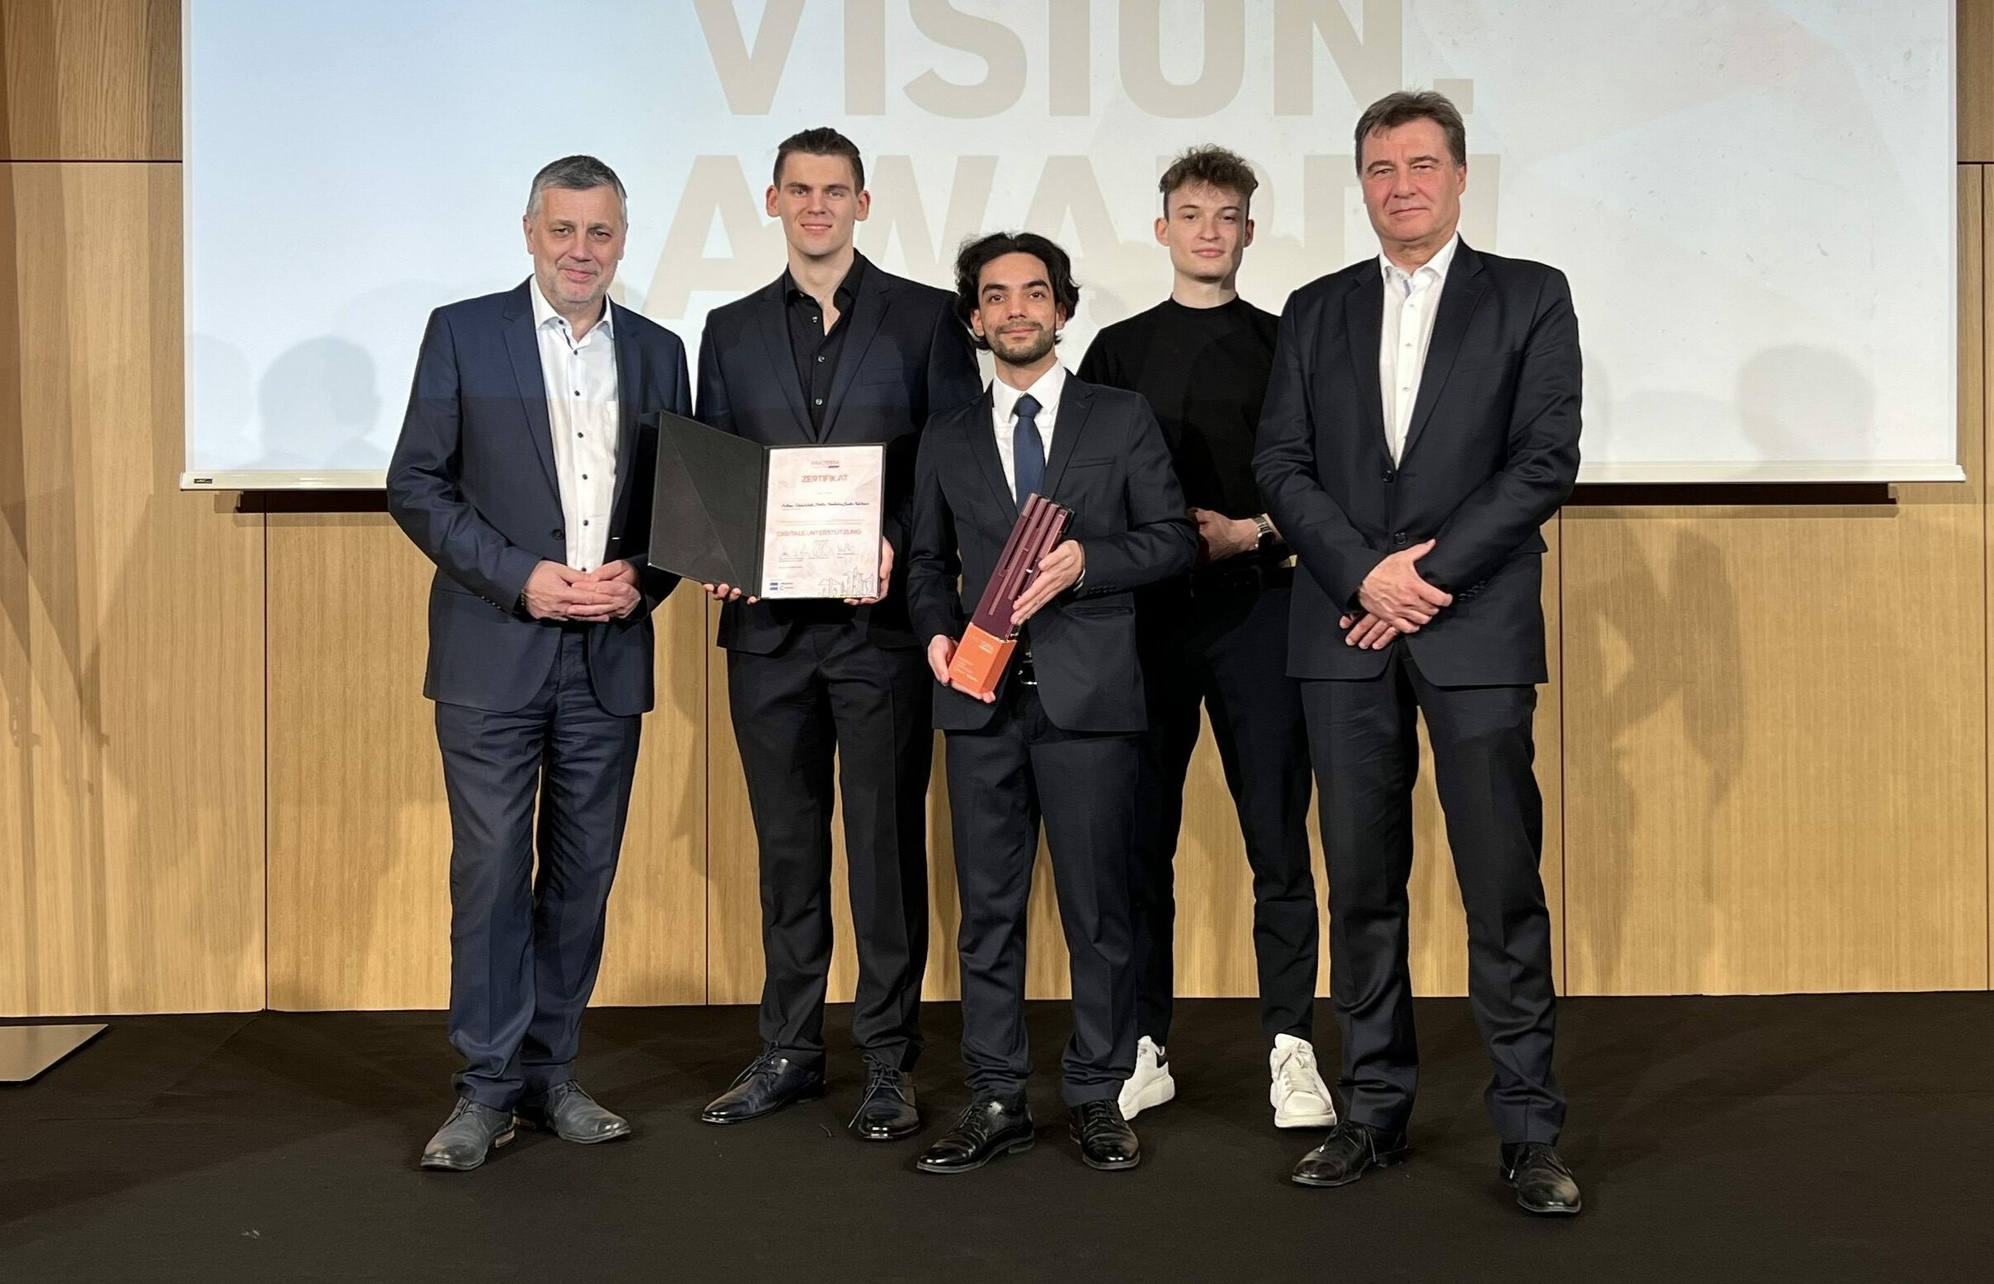
\includegraphics[width=1\textwidth]{pics/Immotopia-2023.jpg}
    \caption{Immotopia Innovation Award 2023}
    \label{fig:Immotopia2023}
\end{figure}

\begin{itemize}
    \item \textbf{Workshop Präsentationstechnik (HTL Leonding):}
          \begin{itemize}
              \item \textbf{16. Februar 2023}
          \end{itemize}
\end{itemize}

Für den Pitch am Ende des mPreneur Social Mobile Entrpreneurship in Ohrid nahm Arsham Edalatkhah an etwa 6 bis 8 Online-Trainingseinheiten zur Vorbereitung mit drei Jurymitgliedern des World Summit Award teil. Er lernte viel über die Kunst des Pitchings und beschloss daher, eines der WSA-Jurymitglieder einzuladen, einen 120-minütigen Workshop über Präsentationstechniken zu halten.

Der Präsentationstechnik-Workshop wurde von Arsham Edalatkhah organisiert, um den Horizont der SchülerInnen der HTL Leonding zu erweitern und ihnen zu helfen, qualitativ hochwertige Präsentationen in verschiedenen Situationen vorzubereiten. Der Inhalt des Workshops besteht aus dem über 10-jährigen Wissen und der Erfahrung des Gastgebers auf dem Gebiet der Präsentation und des Pitchings.

\begin{itemize}
    \item \textbf{ICT4D.at Project-Forge Workshop 2022 (Wien):}
          \begin{itemize}
              \item \textbf{30. November 2022}
          \end{itemize}
\end{itemize}

Die Project-Forge (Quelle: \cite{ict4d-project-forge-report} ) ist ein einzigartig strukturierter Workshop, bei dem mehrere Mitglieder und zusätzliche Gäste zusammenkommen, um eine Reihe von verschiedenen ICT4D.at-Projekten aus unterschiedlichen Regionen der Welt zu diskutieren.

Ziel ist es, durch die offene Diskussion der Projekte, den Austausch von Tipps, das Hinterfragen und Kommentieren des Prozesses die Möglichkeit zu schaffen, den bestehenden Ideen einen zusätzlichen Wert zu verleihen und die Visionen der einzelnen Projekte zu schärfen.

Aufgrund des Erfolges der Nochba App beim vergangenen ICT4D.at Wettbewerb wurde das Nochba Team auch zu dieser Veranstaltung eingeladen. Das Projekt Nochba wird im Jahr 2023 ein Gastgeberprojekt für die Diskussionen sein.

Das Bild (siehe Abbildung \ref{fig:Project-Forge-Workshop-2022}) zeigt eine Diskussionsrunde während des ICT4D.at Project-Forge Workshops 2022 in Wien

\begin{figure}[H]
    \centering
    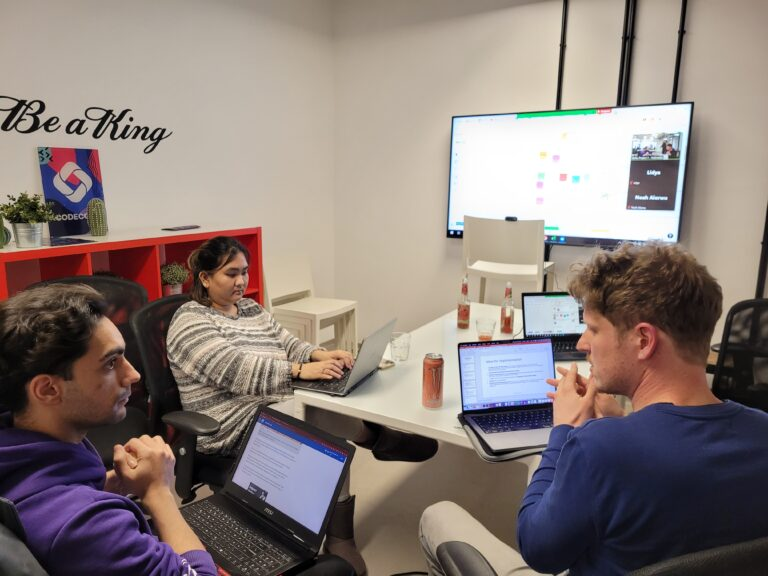
\includegraphics[width=1\textwidth]{pics/Project-forge-01.jpg}
    \caption{ICT4D.at Project-Forge Workshop 2022 (Wien)}
    \label{fig:Project-Forge-Workshop-2022}
\end{figure}

\begin{itemize}
    \item \textbf{UNESCO Internet4Trust Konferenz 2023 (Paris):}
          \begin{itemize}
              \item \textbf{23. Februar 2023}
          \end{itemize}
\end{itemize}

Die von der UNESCO organisierte Internet4Trust-Konferenz (Quelle: \cite{unesco-internet-conference-programme} ) ist eine Veranstaltung zur Förderung von Vertrauen, Sicherheit und Gleichberechtigung im digitalen Raum. Die Konferenz dient als Plattform für den Dialog und die Zusammenarbeit zwischen verschiedenen Stakeholder, darunter Regierungen, Unternehmen des privaten Sektors, Organisationen der Zivilgesellschaft und Lehranstalten.

Das Hauptziel der Internet4Trust-Konferenz besteht darin, die Herausforderungen und Chancen zu diskutieren, die mit dem Aufbau eines vertrauenswürdigen digitalen Umfelds verbunden sind. Dazu gehören Diskussionen über Themen wie Datenschutz, Sicherheit, digitale Kompetenz und die moralische Anwendung von Technologie. Arsham Edalatkhah wurde für die Rolle des WSA Youth Speaker Delegate nominiert, um die Stimme der Jugend während dieser Konferenz zu vertreten, da er am mPreneur Event in Ohrid teilgenommen und sehr gute Ergebnisse erzielt hat. Arsham Edalatkhah nutzte die Gelegenheit auf der UNESCO-Konferenz Internet4Trust 2023 in Paris, um über die vom Team Nochba entwickelte App zu sprechen.

Dies ist ein Bild (siehe Abbildung \ref{fig:unesco-internet4trust-2023}) von Arsham Edalatkhah auf der UNESCO-Bühne zusammen mit dem Moderator Guilherme Canela, Leiter der Abteilung für Meinungsfreiheit und Sicherheit der UNESCO.

\begin{figure}[H]
    \centering
    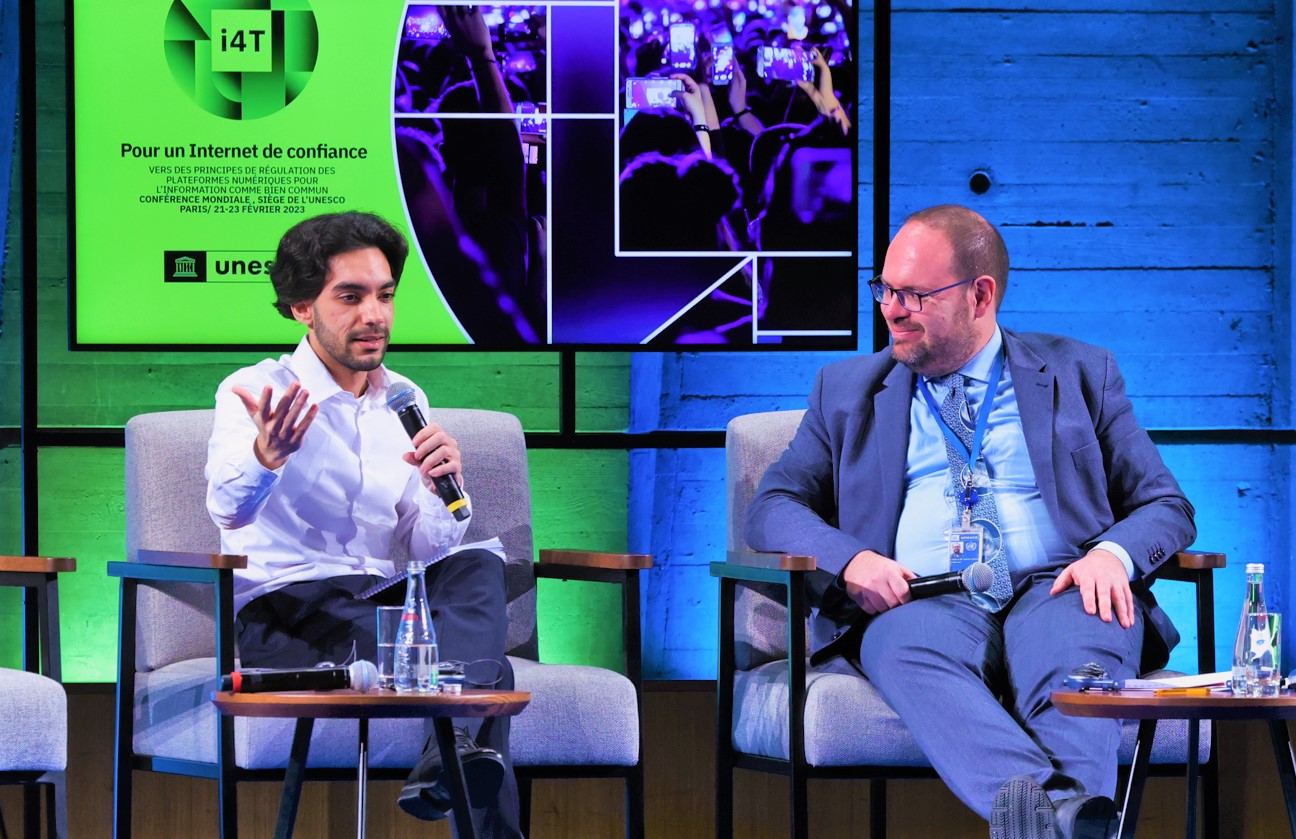
\includegraphics[width=1\textwidth]{pics/unesco-internet4trust-2023.jpg}
    \caption{UNESCO Internet4Trust Konferenz 2023 (Paris):}
    \label{fig:unesco-internet4trust-2023}
\end{figure}

\begin{itemize}
    \item \textbf{Spusu Innovation Award (Wien):}
          \begin{itemize}
              \item \textbf{22. März 2023}
          \end{itemize}
\end{itemize}

Der Spusu Innovation Award (Quelle: \cite{spusu-innovation-award} ) ist ein bedeutendes Preisverleihungsprogramm, das in Wien organisiert wird. Der Spusu Innovation Award wird von Spusu, einem Mobilfunkbetreiber in Österreich, organisiert und gesponsert.

Das Team Nochba erreichte bei diesem Wettbewerb den dritten Platz in der Kategorie soziale Innovation. Hier ist ein Bild des Teams Nochba zusammen mit der Jury und dem Veranstalter des Spusu Innovation Awards 2023 in Wien. [Referenz: Abbildung \ref{fig:spusu-InnovationAward-2023}]

\begin{figure}[H]
    \centering
    \includegraphics[width=1\textwidth]{pics/spusu-InnovationAward-2023.jpg}
    \caption{Spusu Innovation Award 2023 (Wien)}
    \label{fig:spusu-InnovationAward-2023}
\end{figure}

\begin{itemize}
    \item \textbf{World Summit Award (Graz)}
          \begin{itemize}
              \item \textbf{26. bis 28. April 2023}
          \end{itemize}
\end{itemize}

Der World Summit Award (WSA) in Graz ist ein angesehener internationaler Wettbewerb (Quelle: \cite{wsa-global} ) , der hervorragende digitale Innovationen mit einem starken Fokus auf soziale Aspekte auszeichnet und diese unterstützt.

Das Hauptziel des World Summit Award ist es, digitale Innovationen zu identifizieren und zu fördern, die das Potenzial haben, das Leben der Menschen zu verbessern, sich mit aktuellen gesellschaftlichen Herausforderungen auseinanderzusetzen und zur Erreichung der Ziele für nachhaltige Entwicklung der Vereinten Nationen (SDGs) beizutragen.

Das Projekt Nochba hat sich erfolgreich für den hoch geschätzten World Summit Award in der Kategorie \textit{Soziale Innovation} qualifiziert. Grund dafür sind die starken sozialen Aspekte der App und ihr bedeutender Beitrag zu den Zielen für nachhaltige Entwicklung der Vereinten Nationen (SDGs).

Die Teilnahme von Project Nochba am WSA Global Congress wird zweifellos die Sichtbarkeit und den Ruf des Projekts deutlich schärfen und den Weg für eine verstärkte Zusammenarbeit, Investitionen und Unterstützung öffnen, um die Auswirkungen auf die Gemeinschaften weltweit weiter zu verstärken.

\begin{itemize}
    \item \textbf{Hochladen von \textit{Nochba} in den Play Store als Early-Access-App}
          \begin{itemize}
              \item \textbf{22. März 2023}
          \end{itemize}
\end{itemize}

Die Entwicklung einer App umfasst mehrere Phasen, und es muss sichergestellt werden, dass ihre Funktionalität und Benutzerfreundlichkeit den gewünschten Standards entsprechen, bevor sie vollständig veröffentlicht wird. Um dies zu erreichen, hat das Team Nochba die App \textit{Nochba} als Early Access App zu Testzwecken in den Google Play Store hochgeladen. Auf diese Weise konnten die Nutzer wertvolles Feedback geben und Fehler oder Probleme identifizieren, die behoben werden mussten. Im Folgenden finden Sie einen Überblick über die Schritte, die das Team Nochba beim Hochladen von \textit{Nochba} in den Play Store als Early-Access-App unternommen hat:

\begin{itemize}
    \item \textbf{Vorbereiten der App für die Veröffentlichung}
          \begin{itemize}
              \item {Das Team Nochba bereitete die App für die Freigabe vor, indem es sicherstellte, dass sie voll funktionsfähig war und alle erforderlichen Elemente wie Symbole, Screenshots und Materialien für die Präsentation zusammenstellte. Das Team entfernte alle Platzhalter oder Testdaten und bestätigte, dass die App den Richtlinien des Google Play-Entwicklerprogramms und der Vertriebsvereinbarung für Entwickler erfüllt.}
          \end{itemize}
    \item \textbf{Einrichten der App in der Google Play-Konsole}
          \begin{itemize}
              \item {In der Google Play-Konsole richtete das Team Nochba die App ein, indem es die erforderlichen Informationen angab, z. B. den Namen der App, die Standardsprache und den Anwendungstyp, und die entsprechende Preisoption auswählte.}
          \end{itemize}
    \item \textbf{Vorbereiten des App-Store-Listings}
          \begin{itemize}
              \item {Das Team Nochba bereitete die Auflistung der App im Store vor, indem es alle erforderlichen Details bereitstellte, darunter eine Kurzbeschreibung, eine detaillierte Beschreibung, Screenshots, eine Grafik zu den Funktionen und ein App-Symbol, um sicherzustellen, dass die Assets der App den Richtlinien und Spezifikationen von Google Play entsprechen.}
          \end{itemize}
    \item \textbf{Konfigurieren der Inhaltsbewertung der App}
          \begin{itemize}
              \item {Das Team Nochba konfigurierte die Inhaltseinstufung der App, indem es den Fragebogen zur Inhaltseinstufung ausfüllte und so sicherstellte, dass die App der richtigen Zielgruppe angezeigt wurde. In diesem Fall entschied das Team, dass die Nutzer der App mindestens 14 Jahre alt sein sollten, da solche Apps mit diesem Grad an Komplexität und sozialem Aspekt ein gewisses Maß an Reife erfordern, um verantwortungsvoll genutzt zu werden.}
          \end{itemize}
    \item \textbf{Vorbereiten der App für Alpha- oder Beta-Tests}
          \begin{itemize}
              \item {Im Bereich \textit{Testen} der Play Console bereitete das Team Nochba die App für Alpha- oder Betatests vor, indem sie eine Testversion erstellten und die APK- oder App-Bundle-Datei der App hochluden. Außerdem fügten sie alle erforderlichen Informationen hinzu, beispielsweise die Versionshinweise.}
          \end{itemize}
    \item \textbf{Hinzufügen von Testern und Einladung zum Testen der App}
          \begin{itemize}
              \item {Das Team Nochba fügte Tester hinzu und übermittelte ihnen eine Einladung zum Testen der App, indem es die Testmethode (geschlossener oder offener Test) auswählte und den Testern entweder ihre E-Mail-Adressen oder eine URL für den offenen Test zur Verfügung stellte. Das Team informierte die Tester darüber, dass sie Nochba als Early-Access-App über den angegebenen Link aus dem Play Store herunterladen konnten.}
          \end{itemize}
    \item \textbf{Überprüfen und Veröffentlichen der App}
          \begin{itemize}
              \item {Schließlich überprüfte und veröffentlichte das Team Nochba die App. Nachdem sie alle Informationen und Assets überprüft hatten, klickte das Team auf \textit{Überprüfen und veröffentlichen}, um die App zur Überprüfung einzureichen. Der Überprüfungsprozess nahm mehrere Tage in Anspruch. Danach wurde die App im Play Store als Early Access-App zu Testzwecken zur Verfügung gestellt.}
          \end{itemize}
\end{itemize}

Mit diesen Schritten hat das Team Nochba erfolgreich eine Early-Access-App in den Play Store hochgeladen, um wertvolles Feedback von Testern zu sammeln und die Performance und Benutzerfreundlichkeit der App vor dem eigentlichen Start zu verfeinern.

In folgender Abbildung [Referenz: Abbildung \ref{fig:Nochba-GooglePlayStore}] ist ein Screenshot der Nochba-App im Google Play Store zu sehen.

\begin{figure}[H]
    \centering
    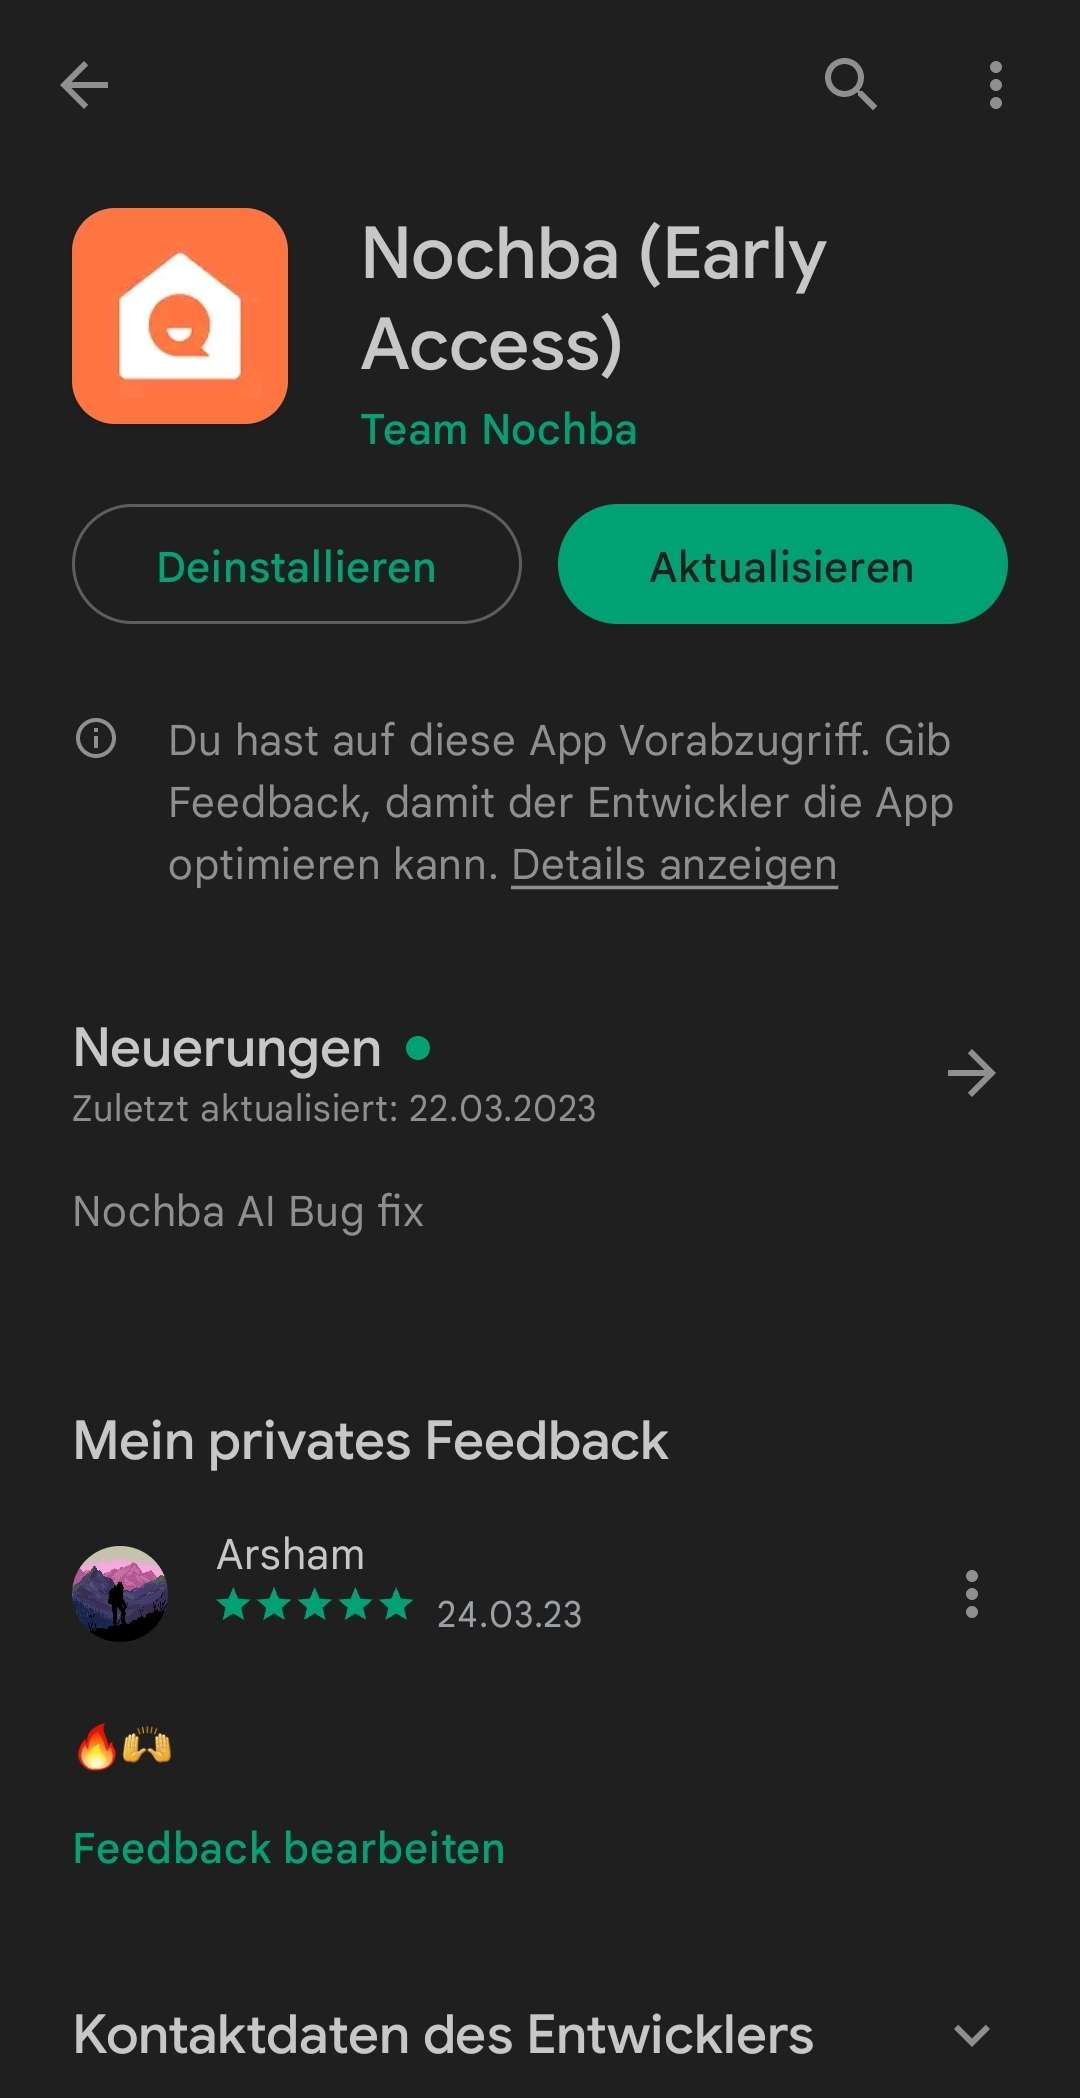
\includegraphics[width=0.3\textwidth]{pics/Nochba-Google_Play_Store.jpg}
    \caption{Screenshot der Nochba-App im Google Play Store}
    \label{fig:Nochba-GooglePlayStore}
\end{figure}

\section{Projektvorgehensmodell}
\subsection{Projektorganisation}

\subsubsection{Discord}
\setauthor{Martin Hausleitner}
Die primäre Kommunikationsplattform zwischen dem Team und den Diplomarbeitbetreuer ist Discord. Da die Arbeit in den Sommerferien 2022 begonnen hat und zu diesem Zeitpunkt Corona-Regelungen galten, musste eine Meeting-Plattform gefunden werden, die sowohl Video- als auch Text-Chat ermöglicht. Aufgrund der Vertrautheit mit Discord und der Tatsache, dass es kostenlos ist, fiel die Entscheidung leicht.

Während der Diplomarbeit wurden über 40 Text-Kanäle erstellt, um alle relevanten Informationen, Notizen und Dokumentation zu speichern. Die Meeting-Notizen wurden jedoch auf ClickUp gespeichert.
\subsubsection{ClickUp}
\setauthor{Martin Hausleitner}
Um das Projekt effizient zu organisieren, wird nicht nur
eine WhatsApp-Gruppe genutzt, sondern auch das
Projektmanagement-Tool ClickUp. Die Entscheidung für ClickUp
fiel leicht, da bereits viele Projektmanagement-Programme
ausprobiert wurden und ClickUp bei den letzten Projekten am
besten abgeschnitten hat. Außerdem ist es sehr intuitiv und
einfach zu erlernen, was von den anderen beiden Teammitgliedern
bestätigt wird.

\begin{figure}[h]
    \centering
    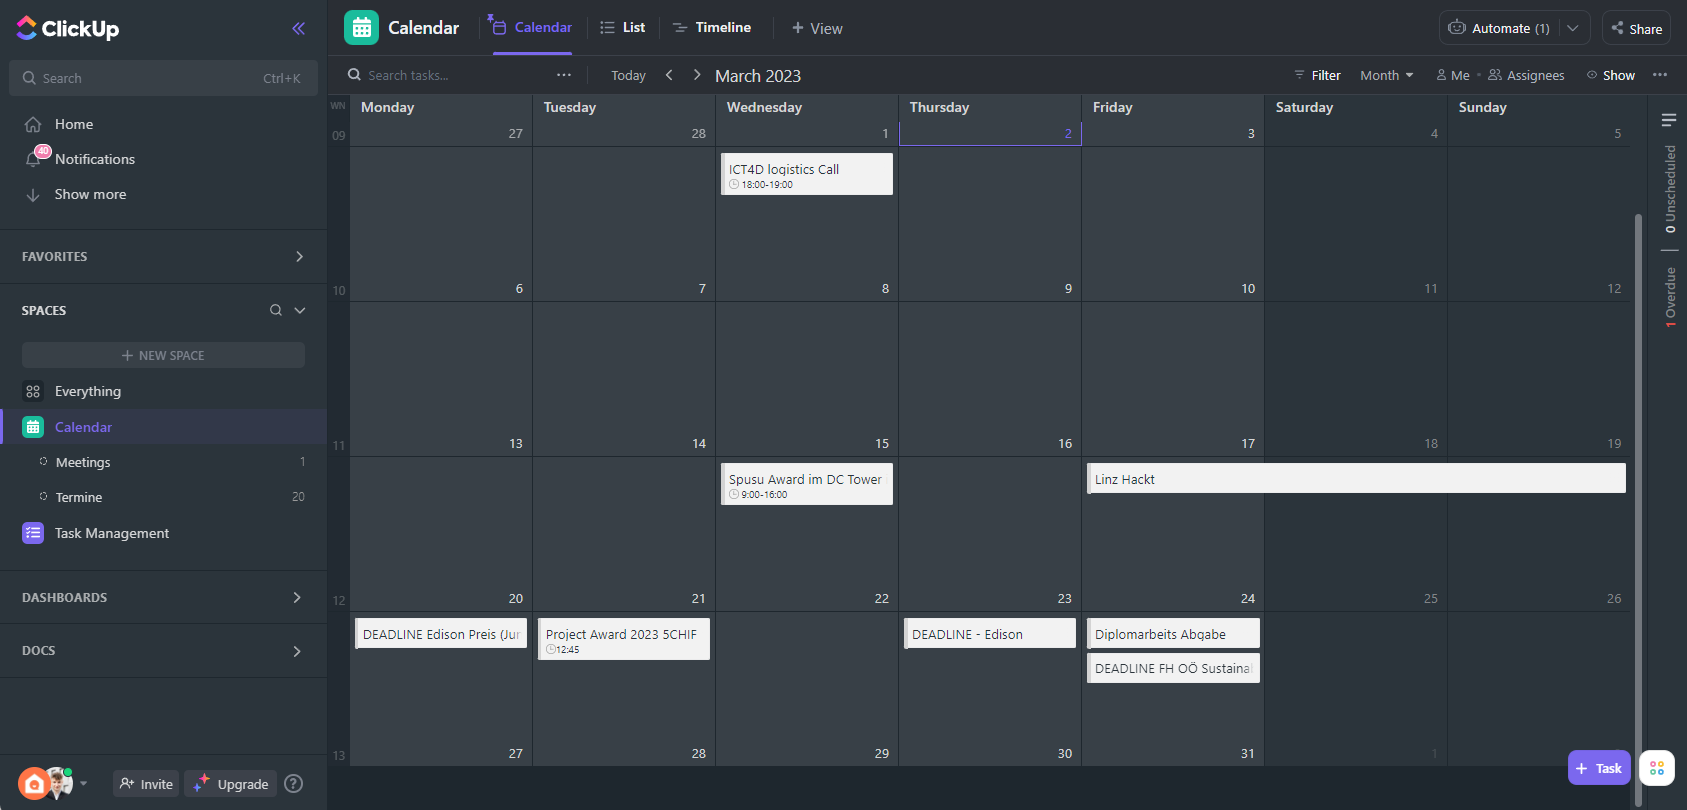
\includegraphics[width=1\textwidth]{./pics/clickup-calender-view.png}
    \caption{ClickUp Dashboard Kalender}
    \label{fig:clickup-calendar}
\end{figure}


In der Diplomarbeit wurden viele Mentoring-Sessions, Meetings mit dem Diplomarbeitbetreuer und weitere Termine wie Wettbewerbe vereinbart. Ohne eine geeignete Methode zur Verwaltung all dieser Termine kann es schnell unübersichtlich werden. Deshalb wurde das Kalender-Feature von ClickUp genutzt, um alle Einträge abzubilden, wie in Abbildung \ref{fig:clickup-calendar} zu sehen ist. Der Kalender wurde automatisch mit den persönlichen Kalendern synchronisiert, wie beispielsweise einem Google Kalender. Dadurch wurden nie Termine verpasst, was insbesondere dem Projektleiter sehr geholfen hat, da er nicht jeden daran erinnern musste, alle Termine in seinem Kalender einzutragen.

Ein weiterer wichtiger Punkt war das Task-Management in dem Projekt. Da im Projekt schnell viele Aufgaben koordiniert werden mussten, war es sinnvoll, alle Aufgaben in einer simplen To-Do-Liste abzubilden. Vor den Semesterferien wurde beispielsweise eine eigene Abteilung für Ferien-Tasks erstellt, um einen Überblick über alle Aufgaben während der Semesterferien zu haben. Obwohl die Tasks-To-Listen nicht aktiv genutzt wurden, war es sehr praktisch, um den Fortschritt zu überwachen und sicherzustellen, dass alles rechtzeitig erledigt wurde.

Zusammenfassend war ClickUp eine große Bereicherung für das
Projektmanagement, da es viel Zeit bei der Verwaltung von
Terminen und Aufgaben gespart hat. Auch die Benutzung als
neuer Benutzer war sehr einfach, sodass keine lange
Einarbeitungszeit nötig war. Besonders faszinierend ist,
dass ClickUp sehr intuitiv ist und viele nützliche Features
bietet.

